




%----------------------------------------------------------------------
\section{Solution Framework}
%----------------------------------------------------------------------

Our solution framework (Figure \ref{Solution framework}) contains two major parts. ``Materialization Part'' takes previous workload as input and perform materializaiton. We first partition previous queries into ``hot'' queries and ``non-hot'' queries based on frequency count of their structures. Cube-Planner and Structure-Planner take ``hot'' queries and ``less hot'' queries as input and select cuboids and substructures (in form of tables) for materialization respectively. ``Future Query Processing Part'' takes future queries as input and generate results. If a future query is of ``hot'' structure we prefer direct aggregation over cuboid materializations in order to efficiently produce results. If no cuboid materialization is useful for a future query, we decompose the query into substructures and produce results by ``joining'' these substructures. In this case, substructure materializations will be used. 

We will discuss ``Materialization Part'' in Section \ref{Materialization Part} and ``Future Query Processing Part'' in Section \ref{Future Query Processing Part}.

\begin {figure}[H]
\centering
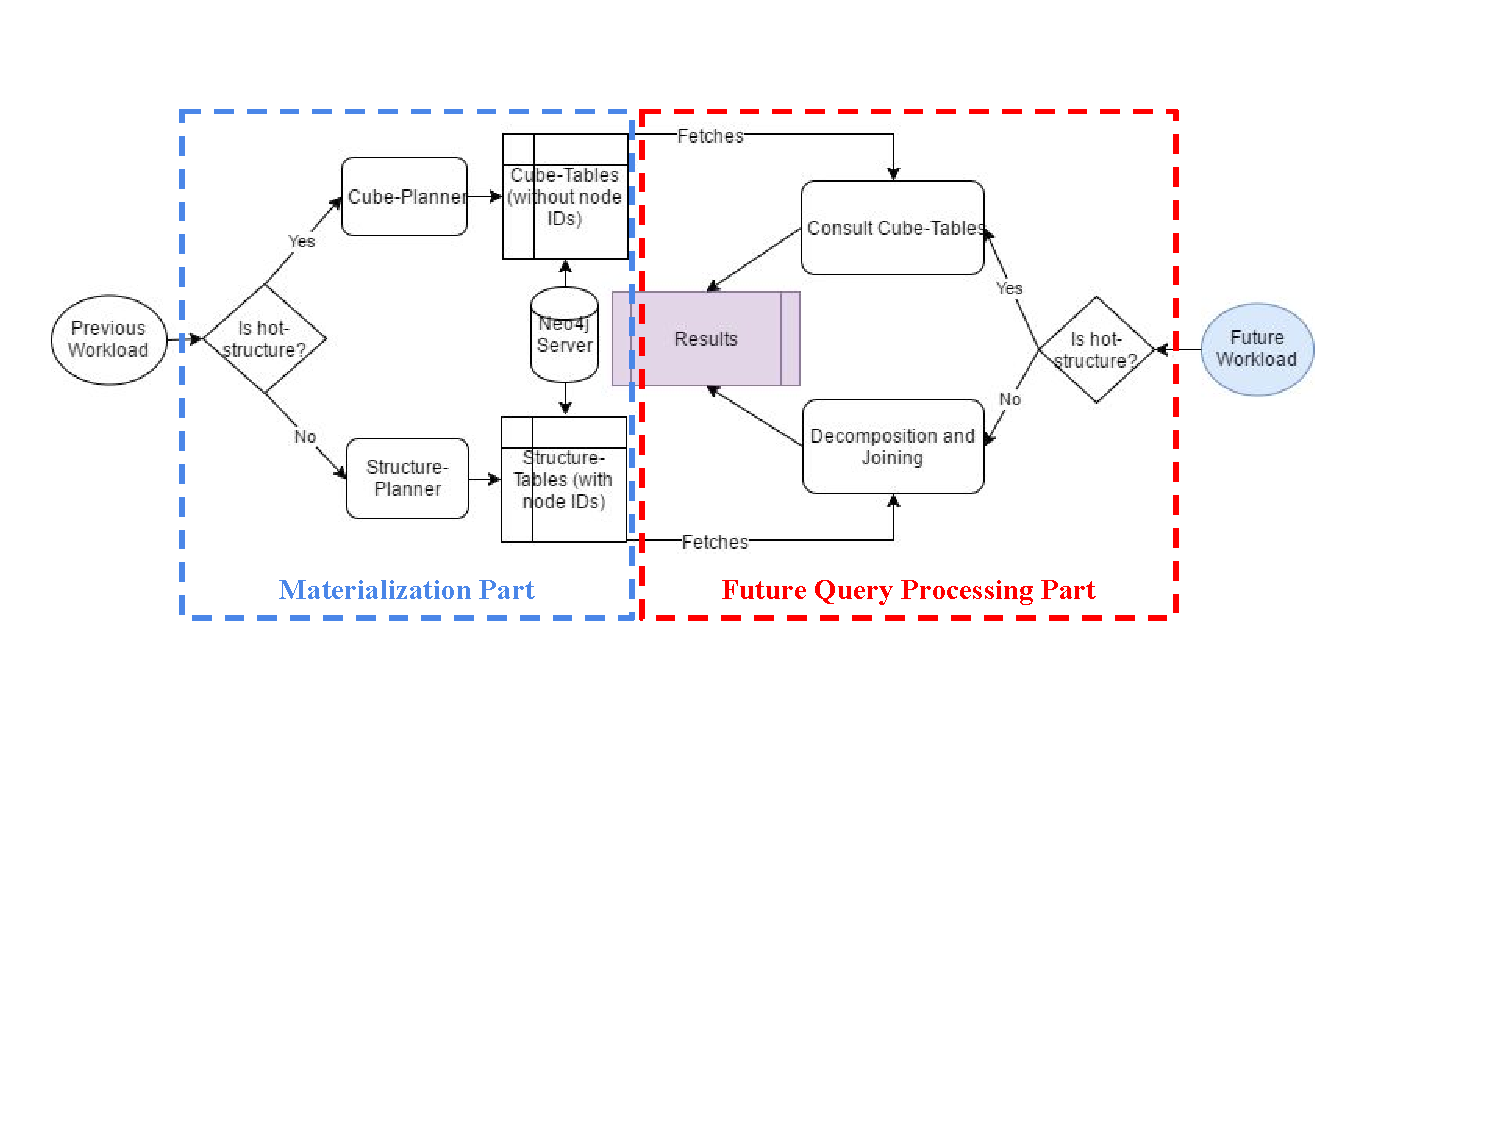
\includegraphics[scale=0.8]{pic/41.pdf}
\caption{Solution framework.}
\label{Solution framework}
\end{figure}


%----------------------------------------------------------------------
\section{Materialization Part}
\label{Materialization Part}
%----------------------------------------------------------------------

%----------------------------------------------------------------------
\subsection{Overview of Materialization Part}
\label{Overview of Materialization Part}
%----------------------------------------------------------------------
In Section \ref{Materialization: Cuboid vs Substructures}, we have discussed about the trade-off between cuboids and substructures. We know that utilization of a cuboid materialization requires future queries to have exactly the same structure as the cuboid. It is wise that we materizalize a cuboid only when we are confident that the structure of a cuboid is likely to be ``hit'' by future queries, because otherwize we may risk wasting space only to materialize cuboids that are rarely "hit". Compared with cuboids, substructures do not have such strict ``structure match'' requirement. A substructure can be used as long as it is structure-wise covered by a future query. 

We make our materialization policy based on such different features of cuboids and substructures. 
We first perform frequency count of previous queries. For queries of structure frequency over a threshold, consider these queries have "hot structure" and pass them to CubePlanner for cuboid selection. For the rest queries with "less hot structure", pass them to StructurePlanner for substructure selection. 

\begin{algorithm}[H]
	\caption{Materialization Overview}
	\LinesNumbered
	\textbf{System setting:} threshold: frequency threshold for hot structures\\ 
	\KwIn{Q: a set of previous queries\\}
	\KwOut{C: a set of materialized cuboids\\ S: a set of materialized substructures}
	
	$CInput \gets \emptyset$ \;
	$SInput \gets \emptyset$ \;
	\ForEach{q \in Q}{
		\eIf{structureFreq(Q, q) $>$ threshold}{
			$CInput \gets CInput \cup \{q\} $\;
		}{	
			$SInput \gets SInput \cup \{q\} $\;
		}
	}
	$C:=materialize(CubePlanner(CInput))$ \;
	$S:=materialize(StructurePlanner(SInput))$\;
\label{alg:PartialMaterialization}
\end{algorithm}
\clearpage

For example, suppose we have the following previous queries and future queries.

\textbf{Previous Workload:}

\begin{itemize}
\item Badge-User, User-Post:Badge.Name,Post.Score,Post.PostTypeId=2

\item User-Comment, Comment-Post: User.UpVotes, Comment.Score, (AVG)Post.Score, Post.PostTypeId=1

\item User-Post, Post-Vote: User.UpVotes, Vote.VoteTypeId

\item User-Post, Post-Tag: (AVG)User.CreationDate\_Year, Tag.TagName

\item User-Comment, Comment-Post: User.ActiveMonth, Post.CreationDate\_Year=2016

\item User-Comment, Comment-Post: User.Age, (AVG)Comment.Score, Post.PostTypeId=2
\end{itemize}


\\
\textbf{Future Workload:}

\begin{itemize}
\item User-Comment, Comment-Post: User.UpVotes, (AVG)Post.Score, Post.PostTypeId

\item User-Comment, Comment-Post: User.Age, Post.PostTypeId

\item User-Post, Post-PostHistory: User.UpVotes, PostHistory.PostHistoryTypeId

\item Badge-User, User-Post:(AVG)Post.Score,Post.PostTypeId=2
\end{itemize}

\par
We count previous queries by structure:

\begin{center}
	\begin{tabular}{ | c | c |}  
		\hline
		Structure	&Frequency	\\ \hline 
		\textbf{User-Comment, Comment-Post} 	&\textbf{3} \\ \hline
		User-Post, Post-Tag 	&1 \\ \hline
		User-Post, Post-Vote	&1 \\ \hline
	\end{tabular}
	\end {center}
\par	
We are confident that \textit{User-Comment, Comment-Post} is a "hot structure". We materialze cuboids over structure \textit{User-Comment, Comment-Post} by passing
\begin{itemize}
\item User-Comment, Comment-Post: User.UpVotes, Comment.Score, (AVG)Post.Score, Post.PostTypeId=1

\item User-Comment, Comment-Post: User.ActiveMonth, Post.CreationDate\_Year=2016

\item User-Comment, Comment-Post: User.Age, (AVG)Comment.Score, Post.PostTypeId=2
\end{itemize}
to Cube-Planner. Cube-Planner will materialize cuboids that benefit processing of future queries (which have \textit{User-Comment, Comment-Post} structure):

\begin{itemize}
\item User-Comment, Comment-Post: User.UpVotes, (AVG)Post.Score, Post.PostTypeId

\item User-Comment, Comment-Post: User.Age, Post.PostTypeId
\end{itemize}
\par
We pass the three remaining queries of "less hot structure" 
\begin{itemize}
\item Badge-User, User-Post:Badge.Name,Post.Score,Post.PostTypeId=2

\item User-Post, Post-Vote: User.UpVotes, Vote.VoteTypeId

User-Post, Post-Tag: (AVG)User.CreationDate\_Year, Tag.TagName
\end{itemize}
to Structure-Planner. Structure-Planner will discover and materialize most useful substructures. In this case StructurePlanner is likely to find \textit{User-Post} as a useful substructure it can be used in joining the result of future query
\begin{itemize}
\item User-Post, Post-PostHistory: User.UpVotes, PostHistory.PostHistoryTypeId
\item Badge-User, User-Post:(AVG)Post.Score,Post.PostTypeId=2
\end{itemize}
%----------------------------------------------------------------------
\subsection{Greedy Selection Framework}
%----------------------------------------------------------------------

 In our solution framework, ``Materialization Selection Problem''(Section \label{sec:Problem Definition}) is managed by Cube-Planner and Structure-Planner. They both adopt a same greedy selection framework. A naive way of solving ``Materialization Selection Problem'' aims at finding best materializations under a space limit $\sigma$.  is to numerate over all possible combinations of cuboids C and substructures S within space limit $\sigma$. But such naive may result in an unacceptable time complexity. What's worse, suppose we find an answer C* and S* from naive way. It is not guaranteed that actual total space cost of C* and S* is lower than $\sigma$ as we make estimations in our calculation. A greedy algorithm is better in terms of efficiency and it allows materializations to be done one by one until space limit $\sigma$ is hit.
 
 We will discuss this greedy selection framework first so that readers have a high-level idea of our selection policy. We use greedy algorithms for cuboid and substructure selection. The idea is to always pick next candidate with highest ratio of margin benefit/space. After a candidate is picked, we re-evaluate benefit of remaining candidates. Re-evaluation is essential as margin benefit of a candidate may be deducted owing to materializaion of a selected candidate. 


\begin{algorithm}[H]
	\caption{Greedy Selection}
	\LinesNumbered  
	\textbf{System setting:} $\sigma$: space limit\\ 
	\KwIn{C: a set of candidates of cuboids or substructures in lattice structure\\ P: A set of previous queries}
	\KwOut{Q: a queue of selected candidates to materialize\\ }
	\ForEach{c \in C}{
		c.space := estimateSpace(c) \;
		c.benefit := estimateMarginBenefit(c, P, Q) \;
		c.score := c.benefit/c.space \;
	} 
	
	\For{$Q.totalsize < \sigma$}{
		selected := c in C with highest score \;  
		Q.offer(selected)\;
		repeat 1-5 \;
	}
\end{algorithm}

Line 1-5 estimates space cost, marginal benefit for future workload, and score for each candidate. We call this parse  "score calculation".

Line 6-10 keeps picking up candidates with highest score one by one until space limit is hit. Notice that each time a candidate is selected, Line 9 refreshes scores for all candidates by repeating 1-5. We call this parse "pick-and-update".   

Cube-Planner and Structure-Planner apply this greedy selection framework by implementation of ``score caculation'' and "pick-and-update". Future users can vary Cube-Planner and Structure-Planner by plug-ins of their own implementation with consideration of their database features. We will introduce how we implement our Cube-Planner and Structure-Planner for Neo4j in the following subsections.
 
%----------------------------------------------------------------------
\subsection{Cube Planner}
%----------------------------------------------------------------------  
As we mentioned, Cube-Planner adopts greedy selection framework. We will first introduce ``Single Cube Planner'' and then ``Holistic Cube Planner''. Input for ``Single Cube Planner'' is previous queries of one same structure while ``Holistic Cube Planner'' deals with previous queries of various structures.
%----------------------------------------------------------------------
\subsubsection{Single Cube Planner}
\label{Single Cube Planner}
%----------------------------------------------------------------------  

Given previous queries of a same structure, we implement  Single Cube Planner from greedy selection framework to select cuboids. 

\begin{algorithm}[H]
	\caption{SingleCubePlanner}
	\LinesNumbered 
	\textbf{System setting:} n: maximum number of cuboids to precompute\\ 
	\KwIn{P: a set of previous queries with a same structure}
	\KwOut{C: an queue of selected cuboids to precompute\\ }
	$Lattice \leftarrow buildLattice(Q)$\;
	\ForEach{query q \in P}{
		$q.time \leftarrow estimateProcessingTime(q)$ \;
	} 
	\ForEach{cuboid \in Lattice}{
		$cuboid.space \leftarrow estimateSpace(cuboid) $\;
		$cuboid.benefit \leftarrow 0$\;
		\ForEach{query q $\in$ P and q.properties $\subseteq$ cuboid.properties}{
			$cuboid.benefit +=max(0, q.time-estimateScanningTime(cuboid))$\;
		}
		$cuboid.score \leftarrow cuboid.benefit/cuboid.space$ \;
	}
	\For{i=1 \emph{\KwTo} n}{
		nextBestCube $\gets$ cuboid in Lattice with highest score \;
		\If{$nextBestCube.score < 0$}{
			break \;
		}
		C.offer(nextBestCube)\;
		\ForEach{cuboid q $\in$ Q and q.dimension $\subseteq$ nextBestCube.dimension }{
			$q.time \gets min(q.time, estimateScanningTime(nextBestCube)) $\;
		}
		repeat 5-12 \;
	}
	
\end{algorithm}
\clearpage

Line 1 builds a lattice over all conbinations of dimensions of all attributes which appeared in previous queries P using classic lattice construction algorithms.

Line 2-4 initializes best-so-far processing time for each previous query by its estimated naive database processing time.

Line 5-12 performs "score calculation" in ``greedy selection framework''. For each cuboid, Line 6 estimates its space. Line 8-10 calculates marginal benefit. Line 8 iterates over previous queries that can be answered by scanning current cuboid. If estimated scanning time is less than a previous query's current best-so-far processing time, we add the difference of two times to the cuboid's total marginal benefit (Line 9).

Line 13-23 performs "pick-and-update" in ``greedy selection framework''. Line 15-17 terminates selection when there is no extra marginal benefit any more. Line 19-22 updates best-so-far processing time for previous queries as a result of current round of selection.

Implementation of functions are listed as follows. Notice that users can implement these functions in their own ways based on their database systems. 

Function \textbf{$estimateProcessingTime(query)$} estimates naive time cost for processing a query by a graph database. Implementation of estimateProcessingTime(query) is database specific as physical storage and execution plans vary among different databases. Since Neo4j provide APIs to see execution plan and estimated intermediate result size, we directly use total size of intermediate results as an estimation of time cost. For example, Figure \ref{fig:4:2} is execution plan provided by Neo4j for query 
\textit{User-Badge, User-Post, Post-Tag: Tag.TagName}. We can see that numbers of ``estimated rows'' for intermediate results are provided. We use  $\displaystyle{\sum ``estimated\_rows''}$ to estimate total processing time cost.

\begin {figure}[H]
\centering
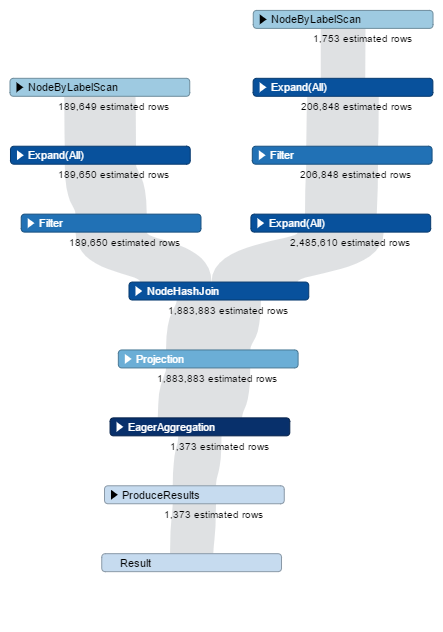
\includegraphics[scale=0.6]{pic/61.png}
\caption{Neo4j's execution plan for query \textit{User-Badge, User-Post, Post-Tag: Tag.TagName}.}
\label{fig:4:2}
\end{figure}

For graph databases where such APIs to see  execution plans and estimated intermediate result sizes are not provided, users need to provide estimation based on their understanding about the database. There are many studies on cost estimations for database operations (joins etc). Users may consider joining (expanding) order \cite{DBLP:conf/pods/Chaudhuri98} and estimation of intermediate result sizes  \cite{DBLP:conf/edbt/SwamiS94} as two important aspects. 

Function \textbf{$estimateScanningTime(cuboid)$} estimates time cost for a scanning cuboid materialization. For cuboid C, we use space cost of C for estimation. 

 $spacePerRow:= 
 \displaystyle{\sum_{p\in C.properties}sizeOf(p)}$
 
$SpaceCost(C):= spacePerRow *  numberOfRows(C)$
 
Here \textit{sizeOf(property type)} refers to standard size of data types. For instance integer type in ``C++'' is 2 byte. \textit{numberOfRows(C)} refers to number of rows of C. A rough estimation is the product of candinalities of all queried properties.  We add a shrinking effect because some conbinations of property values do not exsist in the final result. 
 
$numberOfRows(C):= \displaystyle{\prod_{p\in C.properties}|p|} * shrinking\_factor^{|C.properties|-1}$

%----------------------------------------------------------------------
\subsubsection{Holistic Cube Planner}
%---------------------------------------------------------------------- 

SingleCubePlanner selects cuboids from one lattice of one structure. However input to CubePlanner may consist of previous queries of various structures. CubePlanner performs cuboid selection in a holistic manner by calling SingleCubePlanner for each hot structure and rank cuboids across different lattices (cubes). 

\begin{algorithm}[H]
	\caption{CubePlanner}
	\LinesNumbered 
	\textbf{System setting:} n: maximum number of cuboids to precompute\\ 
	\KwIn{Q: a set of previous queries not nessesarily with a same structure}
	\KwOut{C: a queue of selected cuboids to precompute\\ }
	Group:= GroupByStructure(Q) \;
	\ForEach{group \in Group}{
		group.candidates := SingleCubePlanner(group);
	} 
	
	\For{i=1 \emph{\KwTo} n}{
		selectedGroup := group in Group with highest group.candidates.top().score \; 
		C.offer(selectedGroup.poll())\;
	}
	
\end{algorithm}
\clearpage

Line 1 partitions Q by structure. Each partition consists of previous queries of a same structure, which will be passed to a SingleCubePlanner.

Line 2-4 performs cuboid selection in each partition using SingleCubePlanner. An ordered queue of candidates is generated by each SingleCubePlanner.

Line 5-8 repeatedly checks current top candidate for each partition and picks out the best candidate among them.   

%----------------------------------------------------------------------
\subsection{Structure Planner}
\label{Structure Planner}
%----------------------------------------------------------------------
Like Cube Planner, Structure Planner also adopts ``greedy selection framework''.

\begin{algorithm}[H]
	\caption{StructurePlanner}
	\LinesNumbered 
	\textbf{System setting:} n: maximum number of substructures to precompute\\ 
	\KwIn{Q: a set of previous queries}
	\KwOut{S: an queue of selected substructures to precompute\\ }
	$Lattice \leftarrow buildSubstuctureLattice(Q)$\;
	\ForEach{q \in Q}{
		$q.coveredSubstructres:= \emptyset $\;
	} 
	\ForEach{substructure \in Lattice}{
		$substructure.space \leftarrow estimateSpace(substructure) $\;
		$substructure.benefit \leftarrow 0$\;
		\ForEach{q $\in$ Q and q.structure $\subseteq$ substructure.structure}{
			$cuboid.benefit +=max(0, benefit(q, substructure, q.coveredSubstructres))$\;
		}
		$substructure.score \leftarrow substructure.benefit/substructure.space$ \;
	}
	\For{i=1 \emph{\KwTo} n}{
		nextBestSubstructre $\gets$ substructure in Lattice with highest substructure.score \;
		\If{$nextBestSubstructre.score < 0$}{
			break \;
		}
		S.offer(nextBestSubstructre)\;
		\ForEach{q $\in$ Q and q.structure $\subseteq$ nextBestSubstructre.structure }{
			$q.coveredSubstructres \gets q.coveredSubstructres \cup \{nextBestSubstructre \} $\;
		}
		repeat 5-12 \;
	}
	
\end{algorithm}
\clearpage

Line 1 builds a lattice over all substructures of previous queries P, using classic lattice construction algorithms. Figure \ref{fig:4:3} shows how a lattice over substructures looks like. Starting from a structure of previous query as root node, a lattice can be constructed recursively by populating descendants from parent nodes through edge removal.

\begin {figure}[H]
\centering
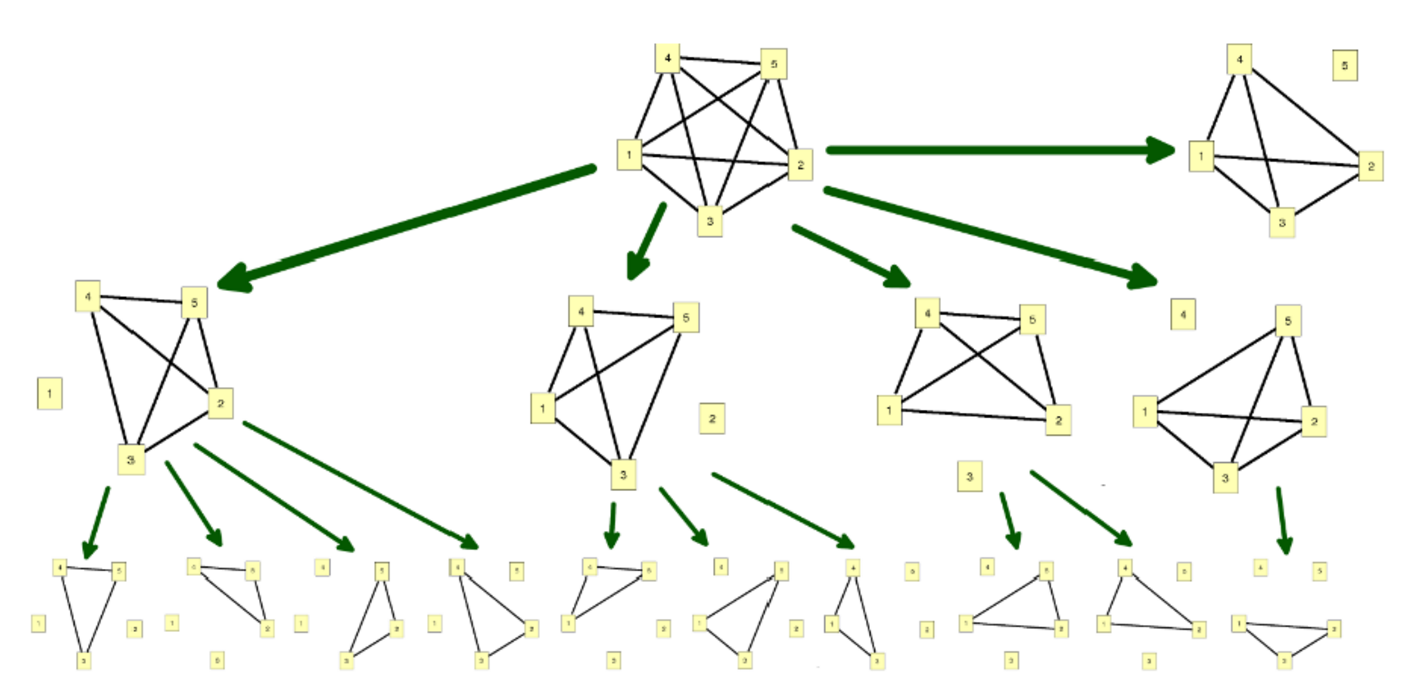
\includegraphics[scale=0.3]{pic/42.png}
\caption{Substructure lattice.}
\label{fig:4:3}
\end{figure}


Line 2-4 initializes covered substructures for each previous query as empty. For a previous query, $coveredSubstructure$ keeps what substructures have been selected so far which are useful for processing this query. It will be updated each time a new substructure is selected.

Line 5-12 performs "score calculation" in ``greedy selection framework''. For each substructure, Line 6 estimates its space. Line 8-10 iterates over all "favored" previous queries (favored by current substructure) and adds on marginal benefit (if any). Here marginal benefit refers to the time saved after adding current substructure to selected  substructures (Line 9).   

Line 13-23 performs "pick-and-update" in ``greedy selection framework''. Line 15-17 terminates selection when there is no marginal benefit any more. Line 19-22 updates covered substructures for previous queries as a result of current round of selection.

Implementation of functions are listed as follows. Again users can implement these functions in their own ways based on their database systems. 
	
Function \textit{estimateSpace(substructure)} returns estimated space cost of a substructure materilization. We use Neo4j's excution plan API to get estimated result size of a substructure.

 Function \textit{benefit(q, substructure, q.coveredSubstructres)} evaluates marginal benefit of substructure to query q when substructures in q.coveredSubstructres have been materialized. We know that execution plan and estimated intermediate result size are provided by Neo4j's API. But such information is on database's naive processing plan. When substructure materialization is used, execution plan (intermediate result) becomes different from naive processing plan. As a result estimation on marginal benefit of a substructure is tricky. We use 
 
 $estimateProcessingTime(q.coveredSubstructres \cup substructure)$ 
 - 
 
 $estimateProcessingTime(q.coveredSubstructres)$
 
 for estimation of marginal benefit of a substructure. We think that this roughly indicates overall improvement of adding $substructure$ to $coveredSubstructres$ as materializations.
 


%----------------------------------------------------------------------
\subsection{ID and Property Selection}
%----------------------------------------------------------------------

Given a substructure picked by Structure Planner, we need to decide on which IDs and attributes should be stored. Keeping all IDs and attributes makes a substructure materialization more informative but increases space cost. We are faced with a tradeoff between space cost and usage potential. Selection on IDs and properties is an important issue. We will use substructure \textit{User-Post, Post-Tag} as an example and discuss different ID and property selection policies.

For IDs, we consider the following two policies.

\begin{itemize}
	\item Policy \#1 keeps IDs of all nodes and edges. This enables ``overlap'' join with  other substructures but increases space cost. For \textit{User-Post, Post-Tag}, if we keep IDs of all nodes and edges, then we can perform join operation with \textit{Badge-User, User-Post}. We call such join an ``overlap'' join as the two substructures have an overlap part which is \textit{User-Post}. Note that we can join the two substructures only when IDs of nodes (User and Post), and edge (edge between User and Post) are stored in both substructures.
	
	\item Policy \#2 keeps IDs of only border nodes. In the example of \textit{User-Post, Post-Tag}, we only save IDs of User and Tag. Compared to Policy \#1, this saves space cost but ``overlap join'' with other substructures is not enabled. Policy \#2 only enables joins on border nodes. For example we may join \textit{User-Post, Post-Tag} with \textit{User-Badge} on their common border node User.
 
	
\end{itemize}


We use Policy \#1 in our implementation. However if keeping IDs of inner nodes and edges overwhelmingly increases result length, it's wise to choose Policy \#2 as space cost becomes dorminant. 

For properties, we consider the following two policies.

\begin{itemize}
	\item Policy \#1 keeps all properties.
	\item Policy \#2 only keeps properties that were queried in previous workloads.
	
\end{itemize}
 
Our suggestion is to consider the proportion of properties which were queried in previous workload over all properties in the data schema. For example, in our experiment only a small proportion of attributes were queried then we choose Policy \#2 as it is a waste of space to keep all properties.


%----------------------------------------------------------------------
\section{Future Query Processing Part}
\label{Future Query Processing Part}
%----------------------------------------------------------------------
Future Query Processing Part aims at processing future queries efficiently using substructure and cuboid materializaitons. When future query q arrives, we first consult materializions of cuboids. If q can be ansered by aggregation over any cuboid materializations, we select the cuboid with minimum space and directly scan over it to produce result of q. If q cannot be answered by any cuboid, we decompose q and use substructures to compose the result of q. 

\begin{algorithm}[H]
	\caption{FutureQueryProcessing}
	\LinesNumbered
	\textbf{System:} C: a set of materialized cuboids\\ S: a set of materialized substructures\\ 
	\KwIn{q: a future query\\}
	\KwOut{r: result of q}
	
	$minspace:= \infty $\;
	mincuboid := NULL \;
	\ForEach{$cuboid \in C$}{
		\If{cuboid.structure = q.structure and q.dimension \subseteq cuboid.dimension}{
			\If{cuboid.space<minspace}{
				minspace := cuboid.space \;
				mincuboid := cuboid \;
			}
		}

	\eIf{mincuboid \not= NULL}{
		r := aggregate(mincuboid, q);
	}{
		r:=Decompose\_Join(q);
	}
	}
\end{algorithm}
\clearpage

Line 4-9 looks up materialized cuboids and find if any cuboid can be used to answer query $q$. If there are multiple useful cuboids we use the cuboid with the smallest scanning cost ($cuboid.space$). Note that $cuboid.space$ was computed in Line 9 in Algorithm SingleCubePlanner in Section \ref{Single Cube Planner}.

Line 10 checks if $q$ can be answered by cuboid materializaiton. If yes we perform aggregation operation over the cuboid (Line 11). Otherwise we need to decompose $q$ into substructures and compose the result (Line 13). 

Function $aggregate(mincuboid, q)$ is classic aggregation operation. We will discuss how function $Decompose\_Join(q)$ is implemented in the following subsections. 

%----------------------------------------------------------------------
\subsection{Substructure Selection}
\label{Substructure Selection}
%----------------------------------------------------------------------

Before discussion on $Decompose\_Join(q)$, we need to first solve a ``Substructure Selection'' problem. In order to decompose a query $q$, we need to consider which substructure materializations we need to use. We need to make dicision when candidate substructures in $S$ overlap. For example suppose $q$ has structure \textit{Badge-User, User-Post, Post-Tag}.

And S consists of substructures 

(1)Badge-User

(2)Badge-User, User-Post 

(3)User-Post, Post-Tag

(4)Post-Tag

(5)User-Post.

Then we may have at least three ways of substructure selection. (1) and (2). (3) and (4).
(1), (4) and (5).

We propose a greedy algorithm for substructure selection. The idea is to always pick up next substructure with highest heuristic. Some exampling heuristics are \#edges of substructure, score calculated in Structure-Planner (Line 11 in Algorithm StructurePlanner), table size etc. 

\begin{algorithm}[H]
	\caption{SelectSubstrucre}
	\LinesNumbered
	\textbf{System:} S: a collection of materialized substructures\\ heuristic: heuristic for ordering S\\
	\KwIn{q: a future query\\}
	\KwOut{V : selected views for future joining\\ uncoveredStruc: structure not covered by selected views\\uncoveredProp: properties not covered by selected views\\}
	uncoveredStruc := q.structure \;
	uncoveredProp:= q.properties \; 
	$coveredStruc:= \emptyset$ \;
	$V:=\emptyset $\;
	\ForEach{$s \in S$ ordered by heuristic}{
		\If{s $\subseteq$ uncoveredStruc and s $\not\subseteq$ coveredStruc}{
			$V := V \cup \{s\}$\;
			$coverdStruc := coveredStruc \cup s.structure$ \;
			uncoveredStruc := uncoveredStruc - s.structure \;
			uncoveredProp := uncoveredProp -s.properties\;
		}
	}
\end{algorithm}
\clearpage

Line 3 initializes $coveredStruc$, which keeps union of selected substructures.

Line 5 starts iteration over substructures using user-defined heuristics. 

Line 6 assures that a candidate substructure that is totally covered by selected substructures will be dequalified. In the above example, suppose we have alreay selected (2), there is no need to select (1) since (1) is totally covered by (2). 

%----------------------------------------------------------------------
\subsection{Decomposation and Join}
\label{Query Decomposition}
%----------------------------------------------------------------------
We have talked about how to select substructure materializations in last subsection. In this part, we will finally discuss how to implement function $Decompose\_Join(q)$ (as in Algorithm FutureQueryProcessing in subsection \ref{Future Query Processing Part}). Besides $Decompose\_Join(q)$, we will also discover two other variations of implementation: $Decompose\_Join_{informative}$ and $Decompose\_Join_{decisive}$. 

%----------------------------------------------------------------------
\subsubsection{Decompose\_Join}
%----------------------------------------------------------------------
Given future query q, we use SelectSubstrucre to select a set of substructure materializaions V. However substructures in V may not completely covers the structure of V. If there is any remaining structure and properties that V does not cover, we need to retrieve them from database. We call such remaining structure and properties fetched from database ``complementary  materials''. After all these components (both materializations and ``complementary  components'') are finally really, we join and aggregate them together to produce final results.

\begin{algorithm}[H]
	\caption{Decompose\_Join}
	\LinesNumbered
	\textbf{System:} S: a collection of materialized substructures\\ heuristic: heuristic for ordering S\\
	\KwIn{q: a future query\\}
	\KwOut{r: result of q}
	$\Sigma \gets \emptyset $\;
	$V, uncoveredStruc, uncoveredProp \gets SelectSubstrucre(q) $\;
	$\Sigma \gets \Sigma \cup V $\;
	Splits:=split(uncoveredStruc, uncoveredProp)\;
	\ForEach{s: Splits}{
		$\Sigma \gets \Sigma \cup \{retrieve(s)\} $\;
	}
	r := join\_aggregate(\Sigma, q)\;
\end{algorithm}

Line 1 initializes $\Sigma$, which maintains a set of all components (materializations and ``complementary  components'') that are needed.

Line 2 selects substructures using SelectSubstructure algorithm. $uncoveredStruc$ and $uncoveredProp$ refer to structures and properties which are not covered by selected substructures. They are ``complementary components'' and will be retrieved from database servers.

Line 4 splits $uncoveredStruc$ and $uncoveredProp$ into connected components. We will retrieve each connected component from database server. Nocice that splitting is nessasary since $uncoveredStruc$ may not be exactly one connected component.

Line 8 joins and aggregates all materials together to produce results. 

Function \textit{split(uncoveredStruc, uncoveredProp)} is implemented by classic connected components detection algorithms.

Function \textit{$materialize(s)$} retrieve ``complementary components'' $s$ from database server.

Function \textit{join($\Sigma$, q)} join tables of $\Sigma$ together and aggregate over properties based on $q$. Joins over multiple tables has been a well-studied topic. Joining order and join technique (hash join etc) are two important aspects on this topic. In our implementation we use hash join and our joining order policy is to keep joining two tables which have minimum sum of table sizes and have common column(s). That is, we tend to select two smaller tables to join.  

%----------------------------------------------------------------------
\subsubsection{$Decompose\_Join_{informative}$}
%----------------------------------------------------------------------
$Decompose\_Join$ retrieve ``complementary components'' from database in a naive manner. We adopt the idea of Semi-Join \cite{DBLP:journals/dr/Ozsoyoglu99} and propose anther way of implementation: $Decompose\_Join_{informative}$. Semi-join takes advantage of ``selection'' effect of natural join. In $Decompose\_Join_{informative}$, we first perform joins over substructures of V. When we retrieve ``complementary components'' from database server, we inform database server with sets of candidate node and edge IDs as a result of joins over V. We name this approach $Decompose\_Join_{informative}$ as instead of naively query ``complementary components'' from database, we try to inform database server with sets of candidate IDs. Database backend only needs to search within candidate IDs. "Informative materialization" helps accerlate retrieval process from backend databases in two aspects. First, since screened out candidate IDs are provided, database backend only needs to iterate through a portion of nodes and edges. This will reduce database processing time. Second, candidate IDs has a filtering effect thus size of retrieval results is likely to be deducted. Thus time of result transmit will be reduced. 

\begin{algorithm}[H]
	\caption{$Decompose\_Join_{informative}$}
	\LinesNumbered
	\textbf{System:} S: a collection of materialized substructures\\ heuristic: heuristic for ordering S\\
	\KwIn{q: a future query\\}
	\KwOut{r: result of q}
	$\Sigma \gets \emptyset $\;
	$V, uncoveredStruc, uncoveredProp \gets SelectSubstrucre(q) $\;
	V^{*}:=join(V)\;
	$\Sigma \gets \Sigma \cup V $\;
	Splits:=split(uncoveredStruc, uncoveredProp)\;
	\ForEach{s: Splits}{
		$\Sigma \gets \Sigma \cup \{retrieve\_{informative}(s, V^{*})\} $\;
	}
	r := join\_aggregate(\Sigma, q)\;
\end{algorithm}
\clearpage

Decompose\_Join performs joining after ``complementary components'' are prepared. Unlike Decompose\_Join, we first join V in Line 3 before retrieval ``complementary components'' from databases in Line 7. Note that substructures in V may reside in multiple connected components. Thus join(V) may result to multiple intermediate join results.

In Line 7, $retrieve\_{informative}(s, V^{*})$ fetches results from databases by passing candidate IDs information (from join result $V^{*}$). Different database server may have different syntax to achievie this. In SQL we may pass candidate IDs using ``WHERE'' statement. Neo4j  supports query with a list of IDs as arguments in ``WHERE'' statement.

------------------
\subsubsection{$Decompose\_Join_{decisive}$}
%----------------------------------------------------------------------
We have mentioned two advantages of $retrieve\_{informative}(s, V^{*})$. However a disadvantage of $retrieve\_{informative}(s, V^{*})$ is an overhead of transport of candidate IDs. We propose a decisive way to evaluate the trade-off between overhead and benefits of $retrieve\_{informative}(s, V^{*})$ and choose between $retrieve\_{informative}(s, V^{*})$ and $retrieve(s)$.

\begin{algorithm}[H]
	\caption{$Decompose\_Join_{decisive}$}
	\LinesNumbered
	\textbf{System:} S: a collection of materialized substructures\\ heuristic: heuristic for ordering S\\
	\KwIn{q: a future query\\}
	\KwOut{r: result of q}
	$\Sigma \gets \emptyset $\;
	$V, uncoveredStruc, uncoveredProp \gets SelectSubstrucre(q) $\;
	V^{*}:=join(V)\;
	$\Sigma \gets \Sigma \cup V $\;
	Splits:=split(uncoveredStruc, uncoveredProp)\;
	\ForEach{s: Splits}{
		\eIf{decide\_informative(s,V^{*})}{
			$\Sigma \gets \Sigma \cup \{retrieve\_{informative}(s, V^{*})\} $\;
		}{
			$\Sigma \gets \Sigma \cup \{retrieve(s)\} $\;
		}
	}
	r := join\_aggregate(\Sigma, q)\;
\end{algorithm}
\clearpage

In Line 7, Function decide\_informative(s,V^{*}) makes decision between $retrieve\_{informative}(s, V^{*})$ and $retrieve(s)$. In our implementation we estimate result sizes two retrieval methods: $retrieve\_{informative}(s, V^{*}).estimatedSize$ and $retrieve(s).estimatedSize$. $retrieve(s).estimatedSize$ can be returned by estimateSpace(substructure) in Algorithm StructurePlanner in subsection \ref{Structure Planner}. We calculate $retrieve\_{informative}(s, V^{*}).estimatedSize$ by the following way:

1. Randomly sample a small number of candidate IDs.  

2. Do $retrieve\_{informative}$ but passing only sampled candidate IDs. We call this a ``trial query''. We want to use ``trial query'' to estimate result length of actual $retrieve\_{informative}(s, V^{*})$. Since we only pass a small number of IDs, time cost of ``trial query'' is small.

3. Using result length of ``trial query'', calculate $retrieve\_{informative}(s, V^{*}).estimatedSize$ proportionally.

After $retrieve(s).estimatedSize$ and $retrieve\_{informative}(s, V^{*}).estimatedSize$ are calculated. We use 

$retrieve(s).estimatedSize - retrieve\_{informative}(s, V^{*}).estimatedSize / sizeOf(candidateIDs)$ and compare the ratio with a threshold to evaluate trade-off and make decision.

